\documentclass{shortart}

\usepackage{amsmath, amssymb, amsthm}
\usepackage{graphicx}
\usepackage{plastex}
\usepackage{tikz-cd}
\usepackage{tikz}

\newcommand\E{\mathbb{E}}
\title{Homology of the \texorpdfstring{$\E_d$}{Ed} operad}
\author{Dexter Chua}

\newtheorem{thm}{Theorem}[section]
\newtheorem{lemma}[thm]{Lemma}
\newtheorem{cor}[thm]{Corollary}

\theoremstyle{definition}
\newtheorem{defi}[thm]{Definition}
\newtheorem{eg}[thm]{Example}

\DeclareMathOperator\Conf{Conf}
\newcommand\R{\mathbb{R}}
\newcommand\N{\mathbb{N}}
\newcommand\Pois{\mathrm{Pois}}
\newcommand\Siop{\mathrm{Siop}}
\newcommand\twotree[2]{
  \begin{tikzpicture}[scale=0.3]
    \draw (0, 0) -- (-0.5, 0.5) node [above=-0.05] {\tiny #1};
    \draw (0, 0) -- (0.5, 0.5) node [above=-0.05] {\tiny #2};
  \end{tikzpicture}
}
\tikzset{circ/.style = {fill, circle, inner sep = 0, minimum size = 3}}
\tikzset{hollow/.style = {draw, fill=white, circle, inner sep = 0, minimum size = 3}}
\newcommand\col{\mathrm{col}}
\begin{document}

\section{Definition of the \texorpdfstring{$\E_d$}{Ed} operad}

\begin{defi}
  $\E_d(n)$ is the space of all $n$ disjoint balls in $D^d$. This is an operad in the usual way.
\end{defi}

As a homotopy type, we have $\E_d(n) \simeq \Conf_n(D^d) \cong \Conf_n(\R^d)$, with the first homotopy equivalence given by shrinking the balls. Recall that
\begin{defi}
  For any topological space $X$, the configuration space $\Conf_n(X) \subseteq X^n$ is the space of $n$ distinct points in $X$, labelled $x_1, \ldots, x_n$.
\end{defi}

The homology of $\Conf_n(\R^d)$ as a group turns out to be pretty easy to compute.

\begin{eg}
  For $n = 2$, it is easy to see that $\Conf_2(\R^d) \simeq S^{d - 1}$. Indeed, by translation, we can assume $x_1 = 0$, and $x_2$ can be any point in $\R^d \setminus \{0\} \simeq S^{d - 1}$.

  A more symmetric way of seeing this is to consider the subspace of $\Conf_2(\R^d)$ consisting of points such that $x_1 = - x_2$ and $\|x_1\| = \|x_2\| = 1$. This is homeomorphic to $S^{d - 1}$ and is a deformation retract of $\Conf_2(\R^d)$ by translation and scaling.
\end{eg}

We focus on the case $d > 2$, so that $S^{d - 1}$ is simply connected. We have fiber sequences
\begin{useimager}
  \[
    \begin{tikzcd}
      \bigvee_{n - 1} S^{d - 1} \ar[r] & \Conf_n(\R^d) \ar[d]\\
      & \Conf_{n - 1}(\R^d)
    \end{tikzcd}
  \]
\end{useimager}
The vertical map forgets the $n$th point and is a fibration. The fiber over a point is $\R^d \setminus \{x_1, \ldots, x_{n - 1}\} \simeq \bigvee_{n - 1} S^{d - 1}$. Inductively, by the Serre spectral sequence, we see that the (co)homology of $\Conf_n(\R^d)$ is free, concentrated in degrees that are multiples of $d - 1$, and the Serre spectral sequence degenerates at $E^2$ for degree reasons.

This tells us the homology and cohomology groups completely as groups, but we lack geometric understanding of all these classes, which is needed to compute the operad structure. What we shall do is to produce explicit (co)homology classes, and this preliminary calculation will tell us when we have found all the classes. For this purpose, all we need are the following two properties:
\begin{enumerate}
  \item $H_{d - 1}(\Conf_n(\R^d))$ and hence $H^{d - 1}(\Conf_n(\R^d))$ is free of rank $\binom{n}{2}$.
  \item The cohomology of $\Conf_n(\R^d)$ is generated as a ring by elements in degree $d - 1$.
\end{enumerate}

In fact, what we will do is to compute the cooperad structure on the cohomology, which we only have to verify in degree $d - 1$, and then dualize to get the operad structure on homology.

\section{Homology}
We produce some homology classes associated to trees.
\begin{defi}
  Let $S \subseteq \{1, \ldots, n\} = \mathbf{n}$. An $S$-tree is a binary tree with a root vertex and leaves labelled by elements of $S$ (each label is used exactly once). We also distinguish between the left and right branches of the binary tree.

  By convention, the term ``vertex'' does not refer to the leaves. Thus, the number of vertices is the number of leaves $ - 1$. We write $|T|$ for the number of vertices of $T$.
\end{defi}

\begin{eg}
  The following is are trees with 1 and 3 vertices respectively:
  \begin{center}
    \begin{tikzpicture}[scale=0.3]
      \draw (0, 0) -- (-0.5, 0.5) node [above=-0.05] {\tiny $i$};
      \draw (0, 0) -- (0.5, 0.5) node [above=-0.05] {\tiny $j$};
    \end{tikzpicture}
    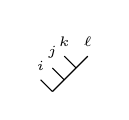
\begin{tikzpicture}[scale=0.3]
      \draw (0, 0) -- (1.5, 1.5) node [above=-0.05] {\tiny $\ell$};
      \draw (0, 0) -- (-0.5, 0.5) node [above=-0.05] {\tiny $i$};
      \draw (0.5, 0.5) -- (0, 1) node [above=-0.05] {\tiny $j$};
      \draw (1, 1) -- (0.5, 1.5) node [above=-0.05] {\tiny $k$};
    \end{tikzpicture}
  \end{center}
\end{eg}

Fix $ 0 < \varepsilon < \frac{1}{3}$. Given an $S$-tree $T$, define a map $P_T: (S^{d - 1})^{\times |T|} \to \Conf_n(\R^d)$ as follows. If $i \in \mathbf{n} \setminus S$, put $x_i$ at some fixed point ``at infinity''. For the rest, we define this by example.

If $T$ is
\begin{tikzpicture}[scale=0.3]
  \draw (0, 0) -- (-0.5, 0.5) node [above=-0.05] {\tiny $i$};
  \draw (0, 0) -- (0.5, 0.5) node [above=-0.05] {\tiny $j$};
\end{tikzpicture}
, we send $\mathbf{v} \in S^{d - 1}$ to the configuration
\begin{center}
  \begin{tikzpicture}
    \draw [dashed] circle (2);
    \node [anchor = north east] {$0$};

    \draw [->] (0, 0) -- (2 / 1.414, 2 / 1.414) node [pos=0.5, anchor = south east, yshift=-2, xshift=2] {$\varepsilon \mathbf{v}$};

    \node [hollow] at (0, 0) {};
    \node [circ] at (2 / 1.414, 2 / 1.414) {};
    \node [anchor = south west] at (2 / 1.414, 2 / 1.414) {$x_i$};
    \node [circ] at (-2 / 1.414, -2 / 1.414) {};
    \node [anchor = north east] at (-2 / 1.414, -2 / 1.414) {$x_j$};
  \end{tikzpicture}
\end{center}
We abbreviate this as $P_{ij}$.

If $T$ is 
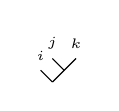
\begin{tikzpicture}[scale=0.3]
  \draw (0, 0) -- (1, 1) node [above=-0.05] {\tiny $k$};
  \draw (0, 0) -- (-0.5, 0.5) node [above=-0.05] {\tiny $i$};
  \draw (0.5, 0.5) -- (0, 1) node [above=-0.05] {\tiny $j$};
\end{tikzpicture}
we send $(\mathbf{v}_1, \mathbf{v}_2)$ to
\begin{center}
  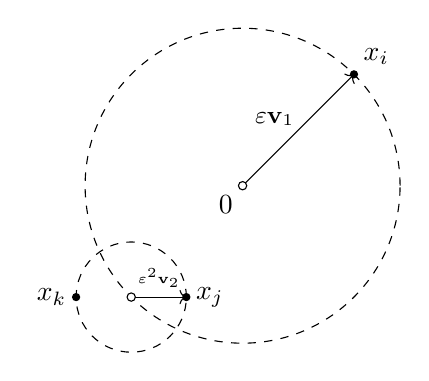
\begin{tikzpicture}
    \draw [dashed] circle (2);
    \node [anchor = north east] {$0$};

    \draw [->] (0, 0) -- (2 / 1.414, 2 / 1.414) node [pos=0.5, anchor = south east, yshift=-2, xshift=2] {\small $\varepsilon \mathbf{v}_1$};

    \node [hollow] at (0, 0) {};
    \node [circ] at (2 / 1.414, 2 / 1.414) {};
    \node [anchor = south west] at (2 / 1.414, 2 / 1.414) {$x_i$};
    \draw [dashed] (-2 / 1.414, -2 / 1.414) circle (0.7);
    \draw [->] (-2 / 1.414, -2 / 1.414) -- +(0.7, 0) node [above, pos=0.5] {\tiny $\varepsilon^2 \mathbf{v}_2$};
    \node [hollow] at (-2 / 1.414, -2 / 1.414) {};

    \node [circ] at (-2 / 1.414 + 0.7, -2 / 1.414) {};
    \node [right] at (-2 / 1.414 + 0.7, -2 / 1.414) {$x_j$};

    \node [circ] at (-2 / 1.414 - 0.7, -2 / 1.414) {};
    \node [left] at (-2 / 1.414 - 0.7, -2 / 1.414) {$x_k$};
  \end{tikzpicture}
\end{center}

The fundamental class of $(S^{d - 1})^{\times |T|}$ gives us a corresponding homology class in $\Conf_n(\R^d)$, which we still call $P_T$.

\begin{thm}
  The classes in $H_*(\Conf_n(\R^d))$ satisfy the relations
  \begin{useimager}
    \[
      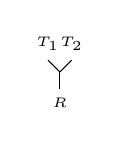
\begin{tikzpicture}[scale=0.3, baseline={([yshift=-.5ex]current bounding box.center)}]
        \draw (0, 0) -- (-0.5, 0.5) node [above=-0.05] {\tiny $T_1$};
        \draw (0, 0) -- (0.5, 0.5) node [above=-0.05] {\tiny $T_2$};
        \draw (0, 0) -- (0, -0.707) node [below=-0.05] {\tiny $R$};
      \end{tikzpicture}
      = (-1)^{d + |T_1| |T_2| (d - 1)}
      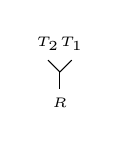
\begin{tikzpicture}[scale=0.3, baseline={([yshift=-.5ex]current bounding box.center)}]
        \draw (0, 0) -- (-0.5, 0.5) node [above=-0.05] {\tiny $T_2$};
        \draw (0, 0) -- (0.5, 0.5) node [above=-0.05] {\tiny $T_1$};
        \draw (0, 0) -- (0, -0.707) node [below=-0.05] {\tiny $R$};
      \end{tikzpicture}
    \]
  \end{useimager}
  \begin{useimager}
    \[
      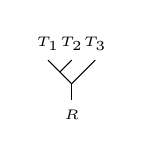
\begin{tikzpicture}[scale=0.3, baseline={([yshift=-.5ex]current bounding box.center)}]
        \draw (0, 0) -- (-1, 1) node [above=-0.05] {\tiny $T_1$};
        \draw (-0.5, 0.5) -- (0, 1) node [above=-0.05] {\tiny $T_2$};
        \draw (0, 0) -- (1, 1) node [above=-0.05] {\tiny $T_3$};
        \draw (0, 0) -- (0, -0.707) node [below=-0.05] {\tiny $R$};
      \end{tikzpicture}
      +
      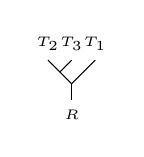
\begin{tikzpicture}[scale=0.3, baseline={([yshift=-.5ex]current bounding box.center)}]
        \draw (0, 0) -- (-1, 1) node [above=-0.05] {\tiny $T_2$};
        \draw (-0.5, 0.5) -- (0, 1) node [above=-0.05] {\tiny $T_3$};
        \draw (0, 0) -- (1, 1) node [above=-0.05] {\tiny $T_1$};
        \draw (0, 0) -- (0, -0.707) node [below=-0.05] {\tiny $R$};
      \end{tikzpicture}
      +
      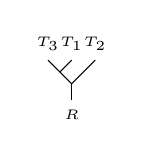
\begin{tikzpicture}[scale=0.3, baseline={([yshift=-.5ex]current bounding box.center)}]
        \draw (0, 0) -- (-1, 1) node [above=-0.05] {\tiny $T_3$};
        \draw (-0.5, 0.5) -- (0, 1) node [above=-0.05] {\tiny $T_1$};
        \draw (0, 0) -- (1, 1) node [above=-0.05] {\tiny $T_2$};
        \draw (0, 0) -- (0, -0.707) node [below=-0.05] {\tiny $R$};
      \end{tikzpicture}
      = 0
    \]
  \end{useimager}
  for any (sub)trees $T_1, T_2, T_3, R$
\end{thm}
The second identity is, of course, the Jacobi identity.

\begin{proof}
  The first identity comes from changing the orientations of $(S^{d - 1})^{\times |T|}$.

  To simplify notation, we only prove the second identity in the case where $T_1, T_2, T_3, R$ are trivial and $n = 3$, i.e.\ we show that
  \begin{useimager}
    \[
      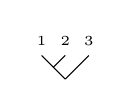
\begin{tikzpicture}[scale=0.3, baseline={([yshift=-.5ex]current bounding box.center)}]
        \draw (0, 0) -- (-1, 1) node [above=-0.05] {\tiny 1};
        \draw (-0.5, 0.5) -- (0, 1) node [above=-0.05] {\tiny 2};
        \draw (0, 0) -- (1, 1) node [above=-0.05] {\tiny 3};
      \end{tikzpicture}
      +
      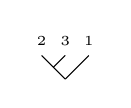
\begin{tikzpicture}[scale=0.3, baseline={([yshift=-.5ex]current bounding box.center)}]
        \draw (0, 0) -- (-1, 1) node [above=-0.05] {\tiny 2};
        \draw (-0.5, 0.5) -- (0, 1) node [above=-0.05] {\tiny 3};
        \draw (0, 0) -- (1, 1) node [above=-0.05] {\tiny 1};
      \end{tikzpicture}
      +
      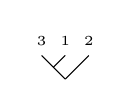
\begin{tikzpicture}[scale=0.3, baseline={([yshift=-.5ex]current bounding box.center)}]
        \draw (0, 0) -- (-1, 1) node [above=-0.05] {\tiny 3};
        \draw (-0.5, 0.5) -- (0, 1) node [above=-0.05] {\tiny 1};
        \draw (0, 0) -- (1, 1) node [above=-0.05] {\tiny 2};
      \end{tikzpicture}
      = 0
    \]
  \end{useimager}
  The general case admits the exact same proof.

  Consider the submanifold of $\Conf_3(\R^d)$ consisting of points satisfying:
  \begin{enumerate}
    \item $\sum x_i = 0$
    \item The perimeter of the triangle spanned by $x_1, x_2, x_3$ is $4\varepsilon + 2 \varepsilon^2$.
    \item The sides of the triangle have length at least $2\varepsilon^2$.
  \end{enumerate}
  One observes that this manifold has three boundary components, achieved when one of the sides have length exactly $2 \varepsilon^2$. One then sees that this component is homotopic to $P_T$ for some $T$ in the identity. For example, the component where the $x_1$--$x_2$ side has length $2 \varepsilon^2$ is homotopic to the first term.
\end{proof}

\begin{defi}
  An $n$-forest is a collection of $S$-trees where each element in $\mathbf{n}$ is used exactly once. 

  If $F = \bigcup T_i$ is an $F$-tree, we define $P_F: (S^{d - 1})^{\times |F|} \to \Conf_n(\R^d)$ in the same way as $P_T$, where the position of $x_k$ is specified by the tree that contains $k$, and the $i$th tree is translated by $(i, 0, 0, \ldots, 0)$.
\end{defi}

\begin{defi}
  Let $\Pois^d(n)$ be the abelian group generated by $n$-forest subject to the (anti)commutativity and the Jacobi identity.
\end{defi}

There is then a map $\Pois^d(n) \to H_*(\Conf_n(\R^d))$, which we will show to be an isomorphism.

\section{Cohomology}
We now produce some cohomology classes of $H_*(\Conf_n(\R^d))$ in degree $d - 1$, which will generate the whole cohomology.

\begin{defi}
  For $i, j \in \{1, \ldots, n\}$, let $\alpha_{ij}: \Conf_n(\R^d) \to \Conf_2(\R^d) \simeq S^{d - 1}$ send $(x_1, \ldots, x_n)$ to $(x_i, x_j)$. Let $a_{ij} \in H^{d - 1}(\Conf_n(\R^d))$ be the pullback of the fundamental class along $\alpha_{ij}$.
\end{defi}

Note that $a_{ij} = (-1)^d a_{ji}$, and $a_{ij}^2 = 0$, since the square of the fundamental class on $S^{d - 1}$ vanishes.

The first claim is that these $a_{ij}$ are dual to the $P_{ij}$.
\begin{lemma}
  Under the homology-cohomology pairing, if $i < j$ and $k < \ell$, then
  \[
    \langle a_{ij}, P_{k\ell}\rangle = \delta_{ik} \delta_{j\ell}.
  \]
  In particular, the set $\{a_{ij}: i < j\}$ is linearly independent and forms a basis of $H^{d - 1}(\Conf_n(\R^d))$, since we know this group is free of rank $\binom{n}{2}$.
\end{lemma}

\begin{proof}
  Consider the composite
  \[
    S^{d - 1} \to \Conf_n(\R^d) \to S^{d - 1}.
  \]
  where the first map picks out $P_{ij}$ and the second $\alpha_{ij}$. The pairing above is given by the degree of this map.

  If $i = k$ and $j = \ell$, then this is the identity map, which has degree $1$. Otherwise, taking $\varepsilon \to 0$ gives a homotopy to the constant map.
\end{proof}

We now know that as a ring, the cohomology of $\Conf_n(\R^d)$ is generated by the $a_{ij}$. We introduce a graphical way to depict products of the $a_{ij}$. Such a product is represented by a graph with vertices $\{1, \ldots, n\}$. Each edge is oriented, and the set of edges is ordered. Multiple edges between vertices is allowed but loops are not.

To depict $a_{ij}$, we take the graph whose only edge is an edge from $i$ to $j$. Products are then represented by unions. For example, $a_{42} a_{43} a_{13}$ is represented by the graph
\begin{center}
  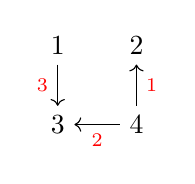
\begin{tikzpicture}
    \node (1) {1};
    \node (2) at (1, 0) {2};
    \node (3) at (0, -1) {3};
    \node (4) at (1, -1) {4};
    \draw [->] (4) -- (2) node [pos=0.5, right] {\scriptsize \color{red} 1};
    \draw [->] (4) -- (3) node [pos=0.5, below] {\scriptsize \color{red} 2};
    \draw [->] (1) -- (3) node [pos=0.5, left] {\scriptsize \color{red} 3};
  \end{tikzpicture}
\end{center}
The numbers on the edges denote the ordering of the edges.

If we swap the ordering of two adjacent edges or reverse an arrow, the class represented picks up a sign of $(-1)^{d - 1}$. Moreover, since $a_{ij}^2 = 0$, any graph with a repeated edge represents $0$.

There is one further relation, which morally is dual to the Jacobi identity.
\begin{lemma}[Arnold]
  \begin{useimager}
    \[
      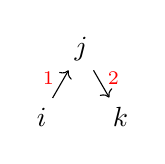
\begin{tikzpicture}[scale=0.5, baseline={([yshift=-.5ex]current bounding box.center)}]
        \node (i) at (-1, 0) {$i$};
        \node (k) at (1, 0) {$k$};
        \node (j) at (0, 1.732) {$j$};

        \draw [->] (i) -- (j) node [pos=0.7, left] {\scriptsize \color{red} 1};
        \draw [->] (j) -- (k) node [pos=0.3, right] {\scriptsize \color{red} 2};
      \end{tikzpicture}
      +
      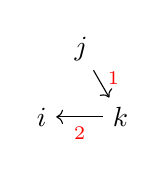
\begin{tikzpicture}[scale=0.5, baseline={([yshift=-.5ex]current bounding box.center)}]
        \node (i) at (-1, 0) {$i$};
        \node (k) at (1, 0) {$k$};
        \node (j) at (0, 1.732) {$j$};

        \draw [->] (j) -- (k) node [pos=0.3, right] {\scriptsize \color{red} 1};
        \draw [->] (k) -- (i) node [pos=0.5, below] {\scriptsize \color{red} 2};
      \end{tikzpicture}
      +
      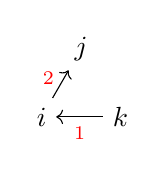
\begin{tikzpicture}[scale=0.5, baseline={([yshift=-.5ex]current bounding box.center)}]
        \node (i) at (-1, 0) {$i$};
        \node (k) at (1, 0) {$k$};
        \node (j) at (0, 1.732) {$j$};

        \draw [->] (k) -- (i) node [pos=0.5, below] {\scriptsize \color{red} 1};
        \draw [->] (i) -- (j) node [pos=0.7, left] {\scriptsize \color{red} 2};
      \end{tikzpicture}
      = 0.
    \]
  \end{useimager}
\end{lemma}

\begin{proof}
  Without loss of generality, we assume $n = 3$ and $(i, j, k) = (1, 2, 3)$. We have to show that
  \[
    a_{12} a_{23} + a_{23} a_{31} + a_{31} a_{12} = 0.
  \]
  We will prove this using the intersection product.

  Recall that if $M^n$ is a compact manifold, then Poincar\'e duality tells us
  \[
    H^k(M^n) \cong H_{n - k}(M^n).
  \]
  Under this isomorphism, the cup product on $H^*(M^n)$ induces a product on $H_*(M^n)$. If $x, y \in H_*(M^n)$ are represented by submanifolds $X, Y$ that intersect transversely, then $x \cdot y$ is represented by $X \cap Y$. This allows for a geometric way to compute the cup product structure of a compact manifold.

  In the case of a non-compact manifold, there are two ways to fix Poincar\'e duality. One is to replace cohomology with compactly supported cohomology, but this is not what we want. Instead, we can replace homology with ``locally finite homology'', also known as Borel--Moore homology, which is given by the homology of the complex of locally finite chains. In particular, arbitrary closed submanifolds of $M^n$ represent a Borel---More homology class.

  Let $\col_i$ be the submanifold of $\Conf_3(\R^d)$ where $x_1, x_2, x_3$ are colinear and $x_i$ is in the middle. This is a submanifold of codimension $d - 1$, and represents a class in $H^{d - 1}(\Conf_3(\R^d))$. We claim that up to a sign, it is $a_{ij} - a_{ik}$ (where $\{j, k\} = \{1, 2, 3\} \setminus \{i\}$).

  To compute the relevant class, we evaluate it on $P_{ij}$, $P_{jk}$ and $P_{ik}$, which is computed by intersecting the relevant submanifolds. It does not intersect $P_{jk}$, because in $P_{jk}$, the point $i$ is at ``infinity'', so cannot be in between $j$ and $k$.

  On the other hand, in $P_{ij}$ and $P_{jk}$, there is exact one point where $i, j, k$ are colinear and $i$ is in the middle, and these points come with opposite signs.

  Now $\col_1$ and $\col_2$ are disjoint, so the represented cohomology classes have zero product. So
  \[
    0 = (a_{12} - a_{13})(a_{23} - a_{21}) = a_{12} a_{23} + a_{23} a_{31} + a_{31} a_{12}.\qedhere
  \]
\end{proof}

\begin{defi}
  We let $\Siop^d(n)$ be the abelian group generated by graphs on $\mathbf{n}$ subject to the previous relations. This is a ring by taking unions.
\end{defi}
There is then a map $\Siop^d(n) \to H^*(\Conf_n(\R^d))$, which we will show to be an isomorphism.

\section{The homology--cohomology pairing}
To compute the homology--cohomology pairing, since $H^*(\Conf_n(\R^d))$ is generated by the $a_{ij}$, it suffices to compute the composites
\[
  \prod_{v \in F} S^{d - 1} \overset{P_F}{\longrightarrow} \Conf_n(\R^d) \overset{\alpha_{ij}}{\longrightarrow} S^{d - 1}
\]
for forests $F$.

If $i$ and $j$ are in different trees, by taking the limit $\varepsilon \to 0$, we see that this map is homotopic to the constant map $(\pm 1, 0, \ldots, 0)$, hence is nullhomotopic. Otherwise, if they meet at $v$, then it is easy to see that up to a sign, this is projection onto the $v$\textsuperscript{th} factor.

\begin{lemma}
  Let $F$ be an $n$-forest and $G$ an $n$-graph. Then under the homology--cohomology pairing, $\langle G, P_F\rangle$ is $\pm 1$ iff
  \begin{enumerate}
    \item For every edge $(i, j)$ in $G$, the corresponding leaves in $F$ are in the same component
    \item The map sending an edge $(i, j)$ to the meet of leaves $\{i, j\}$ gives a bijection between edges of $G$ and vertices of $F$.
  \end{enumerate}
  Otherwise, it is zero.
\end{lemma}
This pairing of forests and graphs is called the \emph{configuration pairing}.

\begin{proof}
  The pairing is the degree of the map
  \[
    \prod_{v \in F} S^{d - 1} \overset{P_F}{\longrightarrow} \Conf_n(\R^d) \overset{\prod\limits_{ij \in G} \alpha_{ij}}{\longrightarrow} \prod_{ij \in G} S^{d - 1}.
  \]
  The lemma is then clear from the previous identification.
\end{proof}

Using this explicit description of the pairing, let us show that the maps $\Pois^d(n) \to H_*(\Conf_n(\R^d))$ and $\Siop^d(n) \to H^*(\Conf_n(\R^d))$ are isomorphisms. We already know that the second map is surjective. Our plan is as follows:
\begin{enumerate}
  \item Write down a spanning set of $\Pois^d(n)$ and $\Siop^d(n)$.
  \item Show that the homology--cohomology pairing pairs these elements perfectly.
  \item Deduce the maps must be injections and $\dim \Pois^d(n) = \dim \Siop^d(n)$, so they are both isomorphisms.
\end{enumerate}

The following lemma follows from applying the Jacobi and Arnold identities:
\begin{lemma}
  $\Pois^d(n)$ is spanned by ``tall'' forests, i.e.\ forests whose trees look like
  \begin{center}
    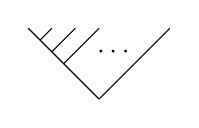
\begin{tikzpicture}[scale=0.3]
       \draw (0, 0) -- (-3, 3);
       \draw (-2.5, 2.5) -- (-2, 3);
       \draw (-2, 2) -- (-1, 3);
       \draw (-1.5, 1.5) -- (0, 3);

       \draw (0, 0) -- (3, 3);
       \node at (0.7, 2) {$\cdots$};
    \end{tikzpicture}
  \end{center}
  where the leftmost vertex has minimal label amongst the leaves. $\Siop^d(n)$ is spanned by ``long graphs'' whose components look like
  \begin{center}
    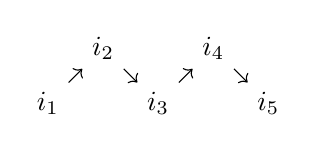
\begin{tikzpicture}[scale=0.7]
      \node (1) at (0, 0) {$i_1$};
      \node (2) at (1, 1) {$i_2$};
      \node (3) at (2, 0) {$i_3$};
      \node (4) at (3, 1) {$i_4$};
      \node (5) at (4, 0) {$i_5$};

      \draw [->] (1) -- (2);
      \draw [->] (2) -- (3);
      \draw [->] (3) -- (4);
      \draw [->] (4) -- (5);
    \end{tikzpicture}
  \end{center}
  where $i_1 < i_2, \ldots, i_5$.
\end{lemma}

\begin{proof}[Hint]
  The first follows form the observation that tall trees are exactly trees where the leftmost vertex is as far away from the root vertex as possible.
\end{proof}

Each of these elements are specified by partitions of $\mathbf{n}$ together with some ordering data.
\begin{lemma}
  The pairing of a tall forest and a long graph is $1$ if they correspond to the same partition, and $0$ otherwise.
\end{lemma}

\begin{cor}
  $\Pois^d(n) \to H_*(\Conf_n(\R^d))$ and $\Siop^d(n) \to H^*(\Conf_n(\R^d))$ are isomorphisms.
\end{cor}

\section{Operad and cooperad structures}
We now describe an operad structure on $\Pois^d$ and the corresponding dual cooperad structure on $\Siop^d$.

Given an $S$-tree, we can produce a bracket expression. For example, we send
\begin{useimager}
  \[
    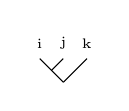
\begin{tikzpicture}[scale=0.3, baseline={([yshift=-.5ex]current bounding box.center)}]
      \draw (0, 0) -- (-1, 1) node [above=-0.05] {\tiny i};
      \draw (-0.5, 0.5) -- (0, 1) node [above=-0.05] {\tiny j};
      \draw (0, 0) -- (1, 1) node [above=-0.05] {\tiny k};
    \end{tikzpicture}
    \mapsto \{\{x_i, x_j\}, x_k\}.
  \]
\end{useimager}
We can then send forests to products of bracket expressions, e.g.
\begin{useimager}
  \[
    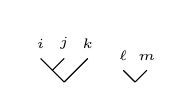
\begin{tikzpicture}[scale=0.3, baseline={([yshift=-.5ex]current bounding box.center)}]
      \draw (0, 0) -- (-1, 1) node [above=-0.05] {\tiny $i$};
      \draw (-0.5, 0.5) -- (0, 1) node [above=-0.05] {\tiny $j$};
      \draw (0, 0) -- (1, 1) node [above=-0.05] {\tiny $k$};
      \begin{scope}[shift={(3, 0)}]

        \draw (0, 0) -- (-0.5, 0.5) node [above=-0.05] {\tiny $\ell$};
        \draw (0, 0) -- (0.5, 0.5) node [above=-0.05] {\tiny $m$};
      \end{scope}
    \end{tikzpicture}
    \mapsto \{\{x_i, x_j\}, x_k\} \cdot \{x_\ell, x_m\}.
  \]
\end{useimager}
The Jacobi identity translates to the usual Jacobi identity of the Lie/Poisson bracket. With the bracket expressions, we can interpret $\Pois^d$ as operad in the usual way by imposing the Leibniz rule
\[
  \{X, Y \cdot Z\} = \{X, Y\} \cdot Z + (-1)^{|X| |Y|} Y \cdot \{X, Z\}
\]

Under the configuration pairing, one checks that this gives the following cooperad structure on $\Siop^d$. To give an operad structure is to give a map $\circ_a: \mathcal{O}(m) \otimes \mathcal{O}(n) \to \mathcal{O}(m + n - 1)$ for every tree of the form
\begin{center}
  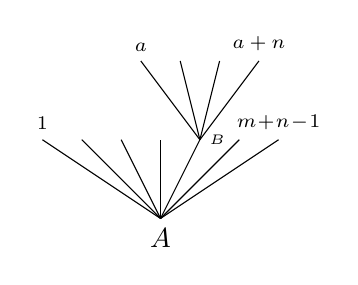
\begin{tikzpicture}
    \foreach \x in {-1.5, -1, -0.5, 0, 0.5, 1, 1.5} {
      \draw (0, 0) -- (\x, 1);
    }
    \node [above] at (-1.5, 1) {\scriptsize $1$};
    \node [above] at (1.5, 1) {\scriptsize $m\! +\! n\! -\! 1$};
    \begin{scope}[shift={(0.5, 1)}]
      \foreach \x in {-0.75, -0.25, 0.25, 0.75} {
        \draw (0, 0) -- (\x, 1);
      }
      \node [above] at (-0.75, 1) {\scriptsize $a$};
      \node [above] at (0.75, 1) {\scriptsize $a + n$};
    \end{scope}
    \node [below] at (0, 0) {$A$};

    \node [right] at (0.5, 1) {\tiny $B$};
  \end{tikzpicture}
\end{center}
where the grafting vertex is the $a$\textsuperscript{th} vertex. Label the two vertices $A$ and $B$. To make $\Siop^d$ a cooperad, we need a map $\Siop^d(m + n - 1) \to \Siop^d(m) \otimes \Siop^d(n)$. This map sends $G$ to $G_A \otimes G_B$, where the edges of $G_1$ and $G_2$ are specified by the following procedure:
\begin{itemize}
  \item For any edge $ij$ of $G$, consider the leaves $i$ and $j$ in the tree above. Let $v$ be the meet of $i$ and $j$ (so that $v = A$ or $B$), and let $J_v(i) = J_v(j)$ be the branches of $v$ over which $i$ and $j$ lie (in this case, one of $J_v(i)$ and $J_v(j)$ will be $i$ or $j$). Then add an edge to $G_v$ from $J_v(i)$ to $J_v(j)$.
\end{itemize}

\begin{thm}
  The map $\Siop^d(n) \to H^*(\Conf_n(\R^d)) = H^*(\E_d(n))$ is an isomorphism of cooperads.
\end{thm}

\begin{cor}
  The map $\Pois^d(n) \to H_*(\Conf_n(\R^d)) = H_*(\E_d(n))$ is an isomorphism of operads.
\end{cor}

\begin{proof}
  Since the cooperad structure is compatible with the product structure, it suffices to show that it preserves $\circ_a$ on $a_{ij}$.

  Consider the composite
  \[
    \E_d(m) \times \E_d(n) \overset{\circ_a}{\longrightarrow} \E_d(m + n - 1) \overset{\alpha_{ij}}{\longrightarrow} S^{d - 1}.
  \]
  Consider the homotopy where at time $t$, the disks in the first factor are scaled by $t$ and the disks in the second factor are scaled by $t^2$. As $t \to 0$, we see that this approaches the projection onto the $v$\textsuperscript{th} factor followed by $\alpha_{J_v(i) J_v(j)}$, as promised.
\end{proof}
\end{document}
